%
% $RCSfile: translator_pattern.tex,v $
%
% Copyright (c) 2001-2004. Christian Heller. All rights reserved.
%
% No copying, altering, distribution or any other actions concerning this
% document, except after explicit permission by the author!
% At some later point in time, this document is planned to be put under
% the GNU FDL license. For now, _everything_ is _restricted_ by the author.
%
% http://www.cybop.net
% - Cybernetics Oriented Programming -
%
% http://www.resmedicinae.org
% - Information in Medicine -
%
% @author Christian Heller <christian.heller@tuxtax.de>
%

\subsection{Translator Pattern}
\label{translator_pattern_heading}

As could be seen in section \ref{biological_reflections_heading}, there is always
a \emph{Translator} that is able to map domain model data to communication model
data (\emph{encode} method) and back (\emph{decode} method). Depending on which
communication medium is used, different translators need to be applied (figure
\ref{translator_classes_figure}).

\begin{figure}[ht]
    \begin{center}
        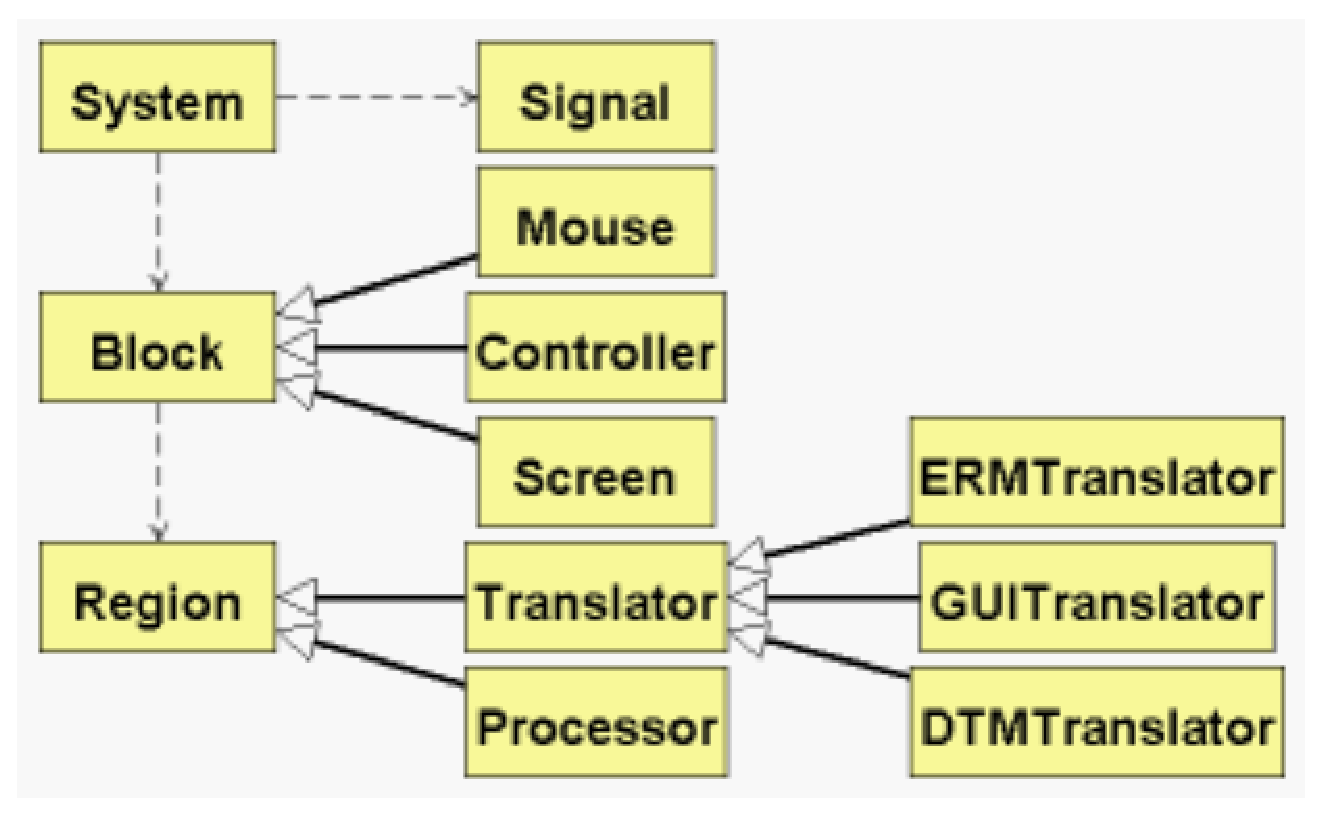
\includegraphics[scale=0.3]{vector/translator_classes.eps}
        \caption{Translator Classes in a UML Class Diagram}
        \label{translator_classes_figure}
    \end{center}
\end{figure}

Every system has exactly one domain model but communication models of arbitrary
type can be added anytime (figure \ref{translator_accessing_models_figure}). Every
translator knows only how to translate between the domain model and a special
communication model. Direct translation between communication models is forbidden
as it would break the flexibility of the whole framework. In other words,
translations always have to be done \emph{via} the domain model.

\begin{figure}[ht]
    \begin{center}
        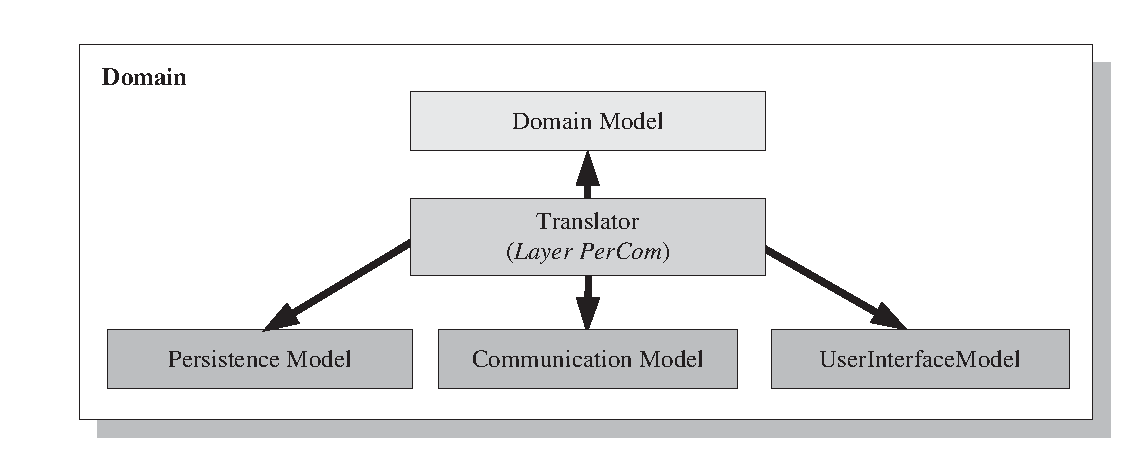
\includegraphics[scale=0.4]{vector/translator_accessing_models.eps}
        \caption{Translator accessing various Models}
        \label{translator_accessing_models_figure}
    \end{center}
\end{figure}

